\documentclass[10pt,xcolor=dvipsnames]{beamer}
\usepackage{amsmath,amssymb,bm}

% Specify theme
\usetheme{default}

% Specify base color
\usecolortheme[named=Black]{structure}

% Specify other colors and options as required
\setbeamertemplate{navigation symbols}{}
%number figures
\setbeamertemplate{caption}{\raggedright\insertcaption\par}
% use latex font
\usefonttheme{professionalfonts}
\usefonttheme{serif}
% more space between blocks

% ------------------- Macros ----------------------
% probability equals sign
\newcommand\peq{\mkern1.5mu{=}\mkern1.5mu}
% likelihood center pipe
\newcommand\lpipe{\mkern1.5mu{|}\mkern1.5mu}
% correlation
\newcommand\lstar{\mkern4mu{\star}\mkern4mu}
% topic sentences
\newcommand{\topic}[1]{\bf{#1}}
% new additions/changes
\newcommand{\new}[1]{{\color{green}#1}}
\newcommand{\del}[1]{{\color{red}\st{#1}}}
% argmin/argmax
\DeclareMathOperator*{\argmin}{\arg\min}
\DeclareMathOperator*{\argmax}{\arg\max}


% Title and author information
\title{Low SNR Multiframe Registration for Cubesats}
\author{Evan Widloski \\ University of Illinois Urbana-Champaign}

\date{2022-09-04}

\begin{document}

% ----- Title -----

\begin{frame}
\titlepage
\end{frame}

\begin{frame}{Outline}
\tableofcontents
\end{frame}

% ----- Introduction -----

\section{Image Registration and the VISORS Mission}

\begin{frame}{Applications and Types of Image Registration}
  \begin{columns}
    \begin{column}{0.5 \textwidth}
      Non-exhaustive list of application areas and tasks
      \begin{itemize}
        \item super resolution
        \item image denoising
        \item image mosaicing
        \item medical image alignment
        \item surveillance
        \item remote sensing
      \end{itemize}

      Classical methods can generally be placed in 2 categories
      \begin{itemize}
        \item area-based
        \item feature-based
      \end{itemize}

    \end{column}

    \begin{column}{0.5 \textwidth}
      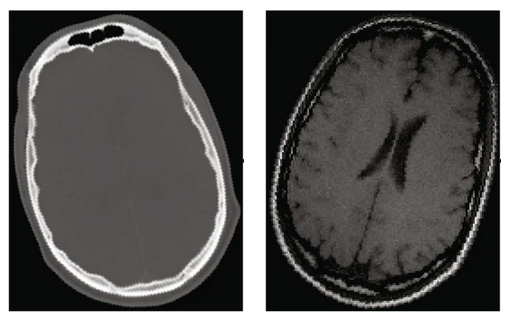
\includegraphics[width=\textwidth]{figures/multimodal.png} \small MRI and CT (Islam 2021)
      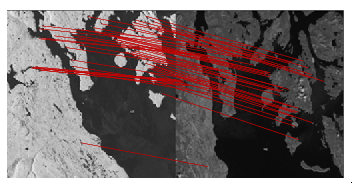
\includegraphics[width=\textwidth]{figures/landmass.png} \small Satellite Imagery (Ma 2017)
      % [Ma 2017]
    \end{column}
  \end{columns}
\end{frame}


\begin{frame}{VISORS Mission}
  \begin{columns}
    \begin{column}{0.5 \textwidth}
      Algorithm conceived for upcoming VISORS mission (2024)
      \begin{itemize}
        \item Studying solar corona
        \item Two cubesats as formation-flying telescope
        \item Optics spacecraft carrying diffractive element known as ``photon sieve''
      \end{itemize}
      Observation model motivates development of new algorithm
      \begin{itemize}
        \item Constant motion between frames in sequence
        \item Low optical efficiency means low SNR on individual frames (below 0 dB)
      \end{itemize}
    \end{column}

    \begin{column}{0.5 \textwidth}
      \begin{overprint}
        \onslide<1>
        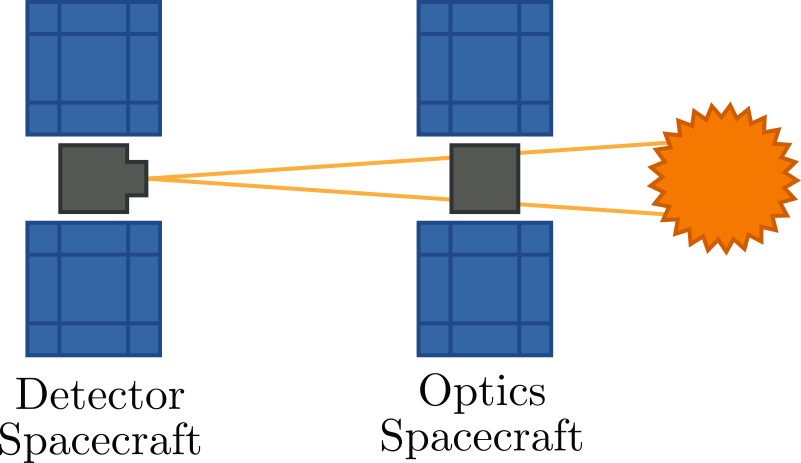
\includegraphics[width=\textwidth]{figures/visors.png}
        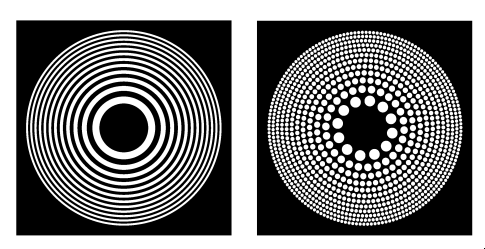
\includegraphics[width=\textwidth]{figures/fresnel.png}
        \\ \small Fresnel lens vs photon sieve
        \onslide<2>
        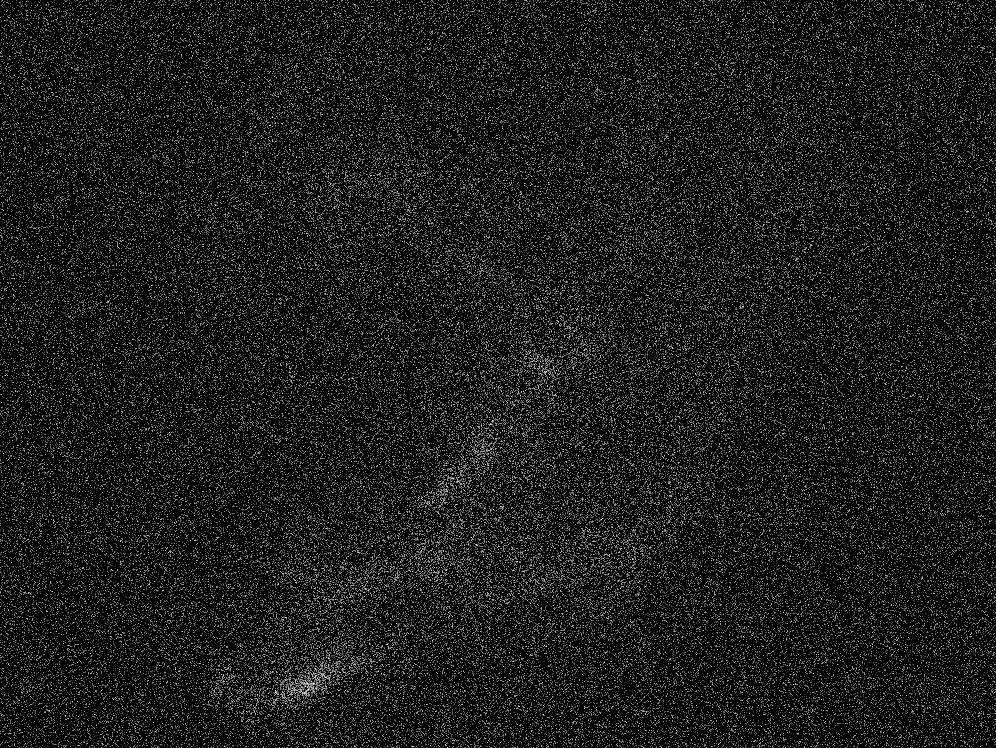
\includegraphics[width=\textwidth]{figures/sample.png}
        \\ \small Simulated VISORS image of corona \\ (-2.5dB) (NASA GSFC, A. Daw)

      \end{overprint}
    \end{column}
  \end{columns}
\end{frame}

%% \begin{itemize}[<+-| alert@+>]

% ----- Observation Model and Algorithm -----

\section{Observation Model and Algorithm}

\begin{frame}{Observation Model}
  \begin{columns}
    \begin{column}{0.5 \textwidth}
      Let $\bm{y}_1, ..., \bm{y}_K \in \mathbb{R}^{N \times N}$ be a sequence of noisy observations where
      $$\bm{y}_k = T_{k\bm{c}}(\bm{\mu}) + \bm{n}_k$$
      \begin{itemize}
        \item $\bm{c} \in \mathbb{R}^2$ - interframe drift
        \item $T(\cdot)$ - translation operator
        \item $\bm{u}$ - ground truth scene
        \item $\bm{n}_k \sim \mathcal{N}(0, \sigma^2)$ - additive Gaussian noise
      \end{itemize}
    \end{column}
    \begin{column}{0.5 \textwidth}
      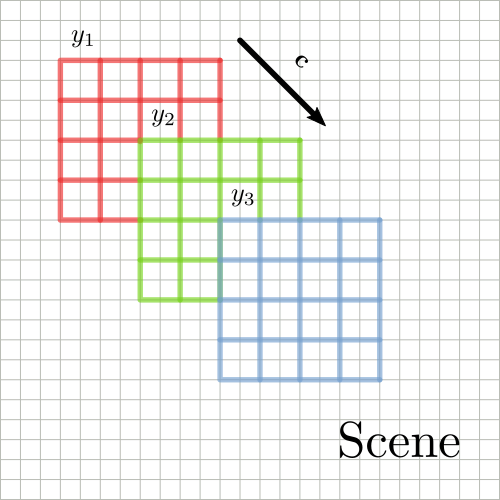
\includegraphics[width=\textwidth]{figures/obs_model.png}
    \end{column}
  \end{columns}

\end{frame}

\begin{frame}{Algorithm}
  \begin{block}{}
    $$
    \hat{\bm{c}} = \arg\max_{\bm{c}} \sum_{m=1}^{K-1} D_m \left( \sum_{k=1}^{K-m} (\bm{y}_k \lstar \bm{y}_{k+m}) \right) [\bm{c}]
    $$
  \end{block}
  \begin{columns}
    \begin{column}{0.5 \textwidth}
      \begin{enumerate}
        \item {\color{BurntOrange} Compute image correlations and sum into groups by degree of separation $m$.}
        \item {\color{OliveGreen}Downsample/downscale each group by degree of separation and sum.}
        \item {\color{MidnightBlue}Find maximum pixel of resulting image for estimating $\bm{c}$}
      \end{enumerate}

    \end{column}

    \begin{column}{0.6 \textwidth}
      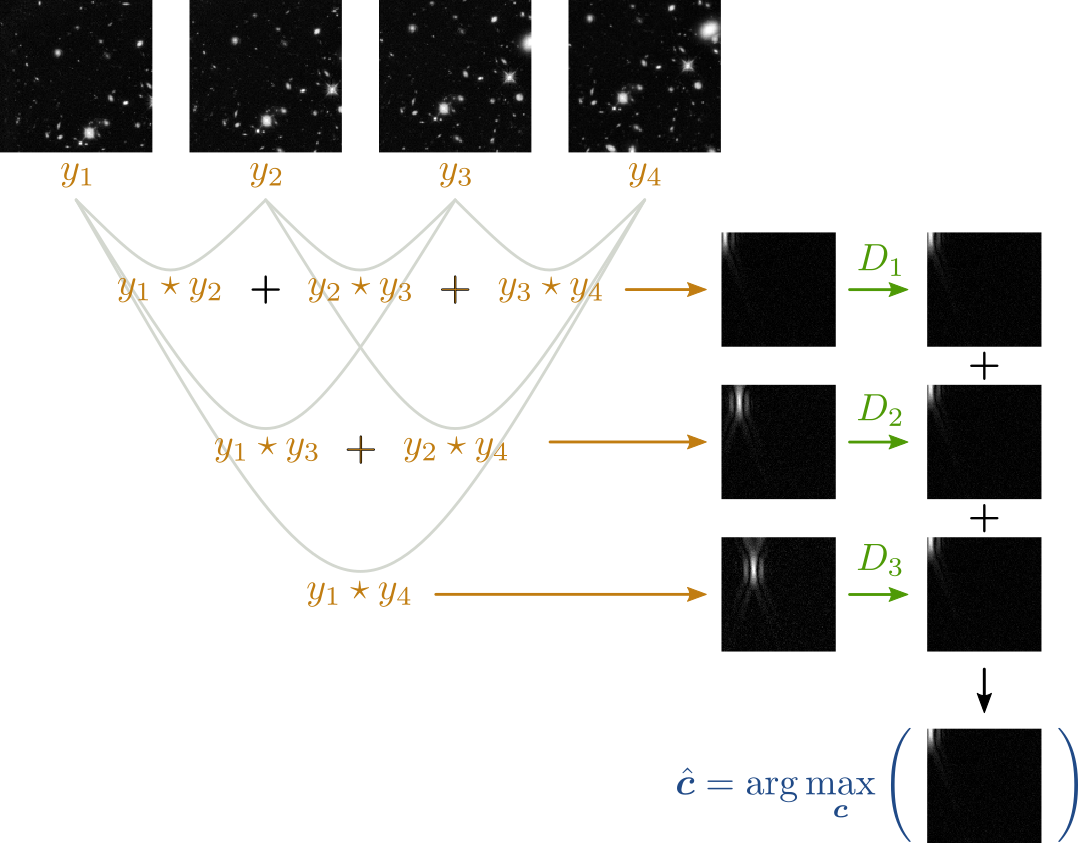
\includegraphics[width=\textwidth]{figures/algorithm_slow.png}
    \end{column}
  \end{columns}
\end{frame}

\begin{frame}{Algorithm - Accelerated}
  \begin{block}{}
    $$
    \hat{\bm{c}} = \argmax_{\bm{c}} \sum_{m=1}^{K-1} D_m \left(
    \mathcal{F}^{-1} \left( \sum_{k=1}^{K-m} \bm{Y}_k \odot \bm{Y}_{k+m} \right)
    \right)[\bm{c}]
    $$
  \end{block}
  \begin{columns}
    \begin{column}{0.5 \textwidth}
      %% $$
      %% \hat{\bm{c}} = \arg\max_{\bm{c}} \sum_{m=1}^{K-1}\sum_{k=1}^{K-m} (\bm{y}_k \lstar \bm{y}_{k+m})[m\bm{c}]
      %% $$
      \begin{enumerate}
        \item {\color{Maroon} Precompute Fourier transform of each frame $\bm{Y}_k$}
        \item {\color{BurntOrange} Compute image correlations and sum into groups by degree of separation $m$.}
        \item {\color{OliveGreen}Downsample/downscale each group by degree of separation and sum.}
        \item {\color{MidnightBlue}Find maximum pixel of resulting image for estimating $\bm{c}$}
      \end{enumerate}

    \end{column}

    \begin{column}{0.6 \textwidth}
      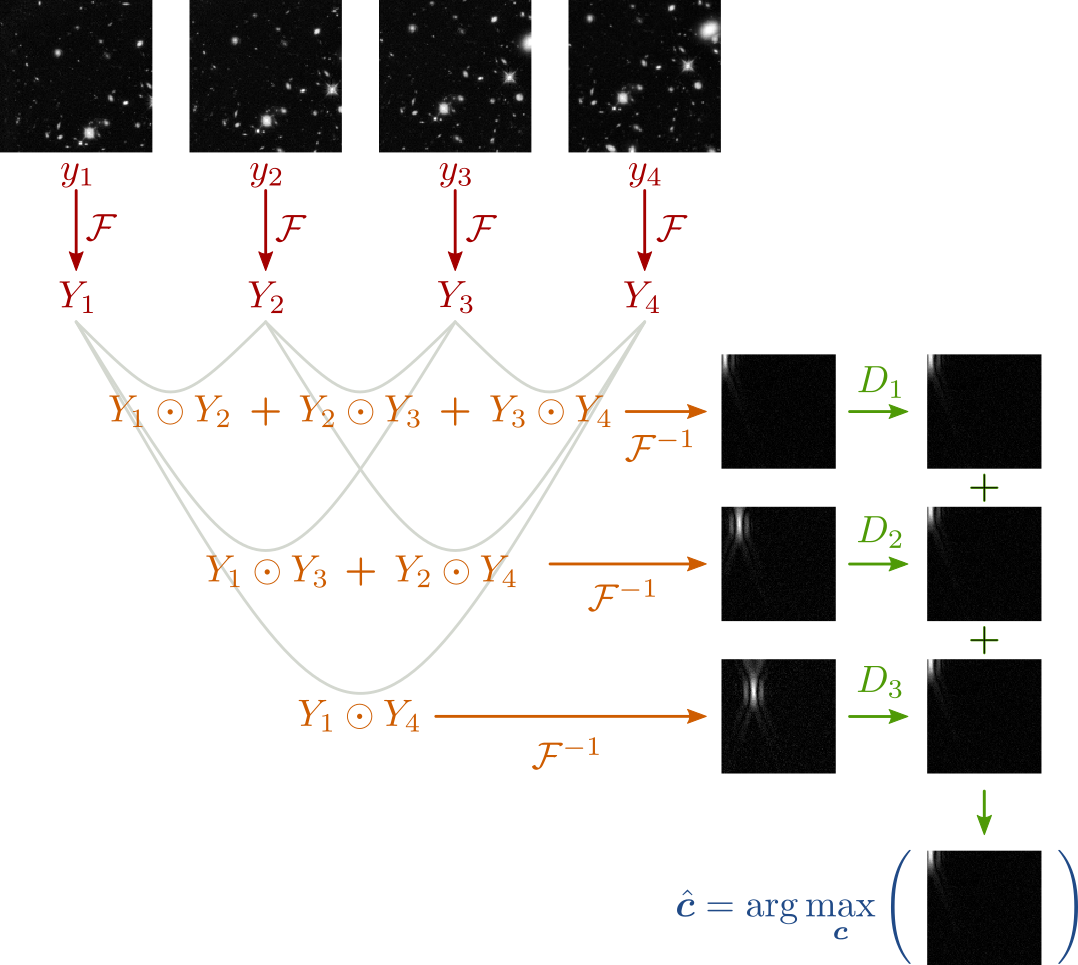
\includegraphics[width=\textwidth]{figures/algorithm.png}
    \end{column}
  \end{columns}
\end{frame}

% ----- ML Optimality -----

\section{ML Optimality}

\begin{frame}{ML Optimality - Likelihood Function}
  $$\bm{y}_k = T_{k\bm{c}}(\bm{\mu}) + \bm{n}_k \hspace{1cm} \bm{n}_k \sim \mathcal{N}(0, \sigma^2)$$
  \begin{itemize}
    \item For simplicity of derivation, assume $T(\cdot)$ is a circular operator.  Approximately true for small $\bm{c}$ relative to image size.
    \item Since noise is independent, the maximum likelihood solution can be written

    \begin{align}
      \hat{\bm{c}}, \hat{\bm{\mu}} &= \argmax_{\bm{c}, \bm{\mu}} \ln \mathcal{L}(\bm{c}, \bm{\mu} \lpipe \bm{y}_1, ..., \bm{y}_K) \nonumber \\
      %% &=\argmax_{c, \mu} \ln \prod_{k=1}^K \prod_{n=1}^N \mathcal{L}(c, \mu \lpipe y_{k,n}) \nonumber \\
      %% &=\argmax_{\bm{c}, \bm{\mu}} \ln \prod_{k=1}^K \prod_{n=1}^N \tfrac{1}{\sigma^2 \sqrt{2 \pi}} \text{exp} \left(- \frac{(\bm{y}_{k,n} - T_{k\bm{c}}(\bm{\mu})_n)^2}{2\sigma^2}\right) \nonumber \\
      &=\argmin_{\bm{c}, \bm{\mu}} \sum_{k=1}^K \sum_{n=1}^N (\bm{y}_{k,n} - T_{k\bm{c}}(\bm{\mu})_n)^2 \label{eq:min}
    \end{align}
  \end{itemize}
\end{frame}

\begin{frame}{ML Optimality - Proof Overview}
  \begin{enumerate}
  \item Derive the expression for likelihood maximization over $\bm{c}$ and $\bm{\mu}$
    $$
      \hat{\bm{c}}, \hat{\bm{\mu}} =
      \argmin_{\bm{c}, \bm{\mu}}
      \underbrace{\sum_{k=1}^K \sum_{n=1}^N (\bm{y}_{k,n} - T_{k\bm{c}}(\bm{\mu})_n)^2}_{\text{cost}(\bm{c}, \bm{\mu})}
    $$
  \item Derive the most likely value for $\bm{\mu}$ as a function of $\bm{c}$
    $$
      \frac{d}{d\mu_j}\left(\text{cost}(\bm{c}, \bm{\mu})\right) = 0 \nonumber
      \hspace{0.5cm} \Longrightarrow \hspace{0.5cm}
      \hat{\bm{\mu}} = \sum_{k=1}^K T_{-k\bm{c}}(\bm{y}_k)
    $$
      $$\text{cost}(\bm{c}, \hat{\bm{\mu}}) = \text{cost}(\bm{c})$$
    \item Show that the log-likelihood solution consists of a sum of downsampled cross correlations

      $$\begin{aligned}
      \hat{\bm{c}} = \argmin_{\bm{c}} \text{cost}(\bm{c})
      &=\argmin_{\bm{c}}\sum_{k=1}^K \sum_{n=1}^N \left(\bm{y}_{k,n} - T_{k\bm{c}}\left(\sum_{l=1}^K T_{-l\bm{c}}(\bm{y}_l)\right)_n\right)^2 \\
      &= ... = \argmax_{\bm{c}} \sum_{m=1}^{K-1} \sum_{k=1}^{K-m} (\bm{y}_k \lstar \bm{y}_{k+m})[m\bm{c}]
      \end{aligned}$$

  \end{enumerate}
\end{frame}

% ----- Numerical Results -----

\section{Numerical Results}

\begin{frame}{Numerical Results - Measurement Noise Sweep}
  $$y_1, ..., y_K \in \mathbb{R}^{250 \times 250}, \text{ 50 trials }$$
  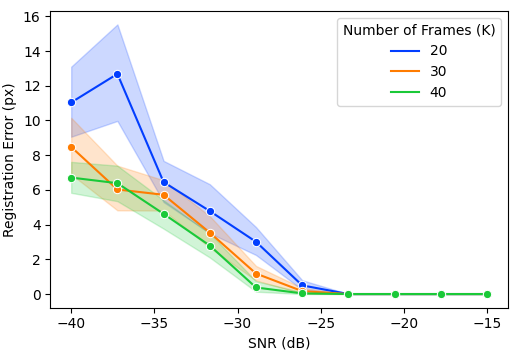
\includegraphics[width=\textwidth]{figures/db_sweep.pdf}
\end{frame}

%% \begin{frame}{Numerical Results - Translational Jitter}
%%   $$
%%   \bm{y}_k = T_{k\bm{c} + \bm{t}_k}(\bm{\mu}) + \bm{n}_k
%%   \hspace{.5cm} \bm{n}_k \sim \mathcal{N}(0, \sigma^2)
%%   \hspace{.3cm} \bm{t}_k \sim \mathcal{N}(0, \sigma_t^2)
%%   $$
%%   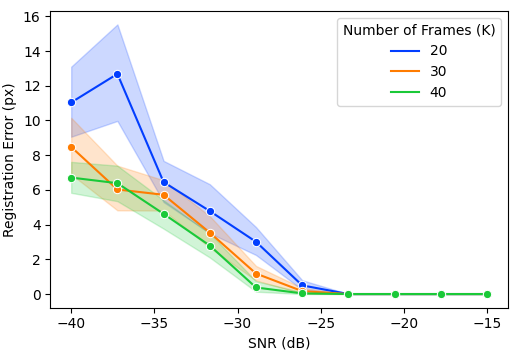
\includegraphics[width=\textwidth]{figures/db_sweep.pdf}
%%   \vspace*{-30ex}
%%   \begin{center}
%%   \large Placeholder Image
%%   \end{center}
%%   \vspace*{30ex}
%% \end{frame}

%% \begin{frame}{Numerical Results - Rotational Jitter}
%%   $$
%%   \bm{y}_k = R_{\theta_k}(T_{k\bm{c}}(\bm{\mu})) + \bm{n}_k
%%   \hspace{.5cm} \bm{n}_k \sim \mathcal{N}(0, \sigma^2)
%%   \hspace{.3cm} \theta_k \sim \mathcal{N}(0, \sigma_{\theta}^2)
%%   $$
%%   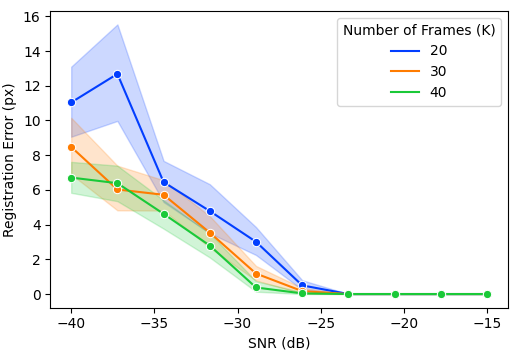
\includegraphics[width=\textwidth]{figures/db_sweep.pdf}
%%   \vspace*{-30ex}
%%   \begin{center}
%%   \large Placeholder Image
%%   \end{center}
%%   \vspace*{30ex}
%% \end{frame}

% ----- Conclusion -----

\begin{frame}{Conclusion}
  \begin{itemize}
    \item Presented ML optimal algorithm for registering sequences of images with constant translational motion
    \item Why you might want to use this:
    \begin{itemize}
      \item Non-iterative, constant-time solution.
      \item Straightforward implementation using only downscale, FFT, and multiply operations
      \item No parameter tuning.
    \end{itemize}

  \item Python implementation available at https://github.com/evidlo/multiml
  \end{itemize}

\end{frame}

% ----- Appendix -----

\section*{Appendix}

\begin{frame}{References}
  \begin{itemize}
    \item Ma, Wenping et al. “Remote Sensing Image Registration With Modified SIFT and Enhanced Feature Matching.” IEEE Geoscience and Remote Sensing Letters 14 (2017): 3-7.
    \item Islam, K.T., Wijewickrema, S. O’Leary, S. A deep learning based framework for the registration of three dimensional multi-modal medical images of the head. Sci Rep 11, 1860 (2021). https://doi.org/10.1038/s41598-021-81044-7
  \end{itemize}
\end{frame}

\end{document}
